\begin{figure}[h]
    \centering
    \begin{subfigure}[b]{0.48\columnwidth}
        \centering
        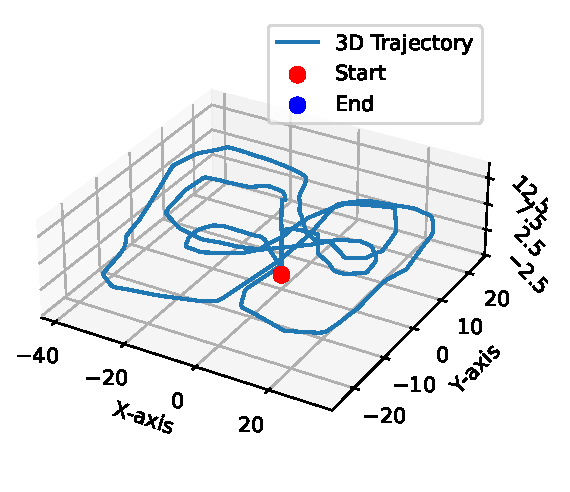
\includegraphics[width=\textwidth]{tex/ch5_airio/figs/pegasus_trajs/pegasus_4_train_test_sorted.pdf}
        \caption{TEST\_1: This trajectory covers a  distance of 558.6$\si{\meter}$ and a total duration of 253.2$\second$, with a peak speed of 4.7 $\si{\meter\per\second}$, an average speed of 2.2 $\si{\meter\per\second}$}
        \label{fig:airio:sub_test1}
    \end{subfigure}
    \hfill
    \begin{subfigure}[b]{0.48\columnwidth}
        \centering
        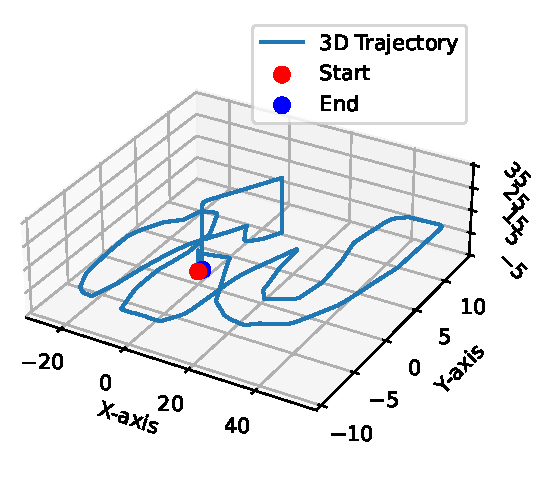
\includegraphics[width=\textwidth]{tex/ch5_airio/figs/pegasus_trajs/pegasus_5_train_test_sorted.pdf}
        \caption{TEST\_2: This trajectory covers a  distance of 316.7$\si{\meter}$ and a total duration of 228.5$\second$, with a peak speed of 4.6 $\si{\meter\per\second}$, an average speed of 1.4 $\si{\meter\per\second}$}
        \label{fig:airio:sub_test2}
    \end{subfigure}

     \vspace{1em}
         \begin{subfigure}[b]{0.48\columnwidth}
        \centering
        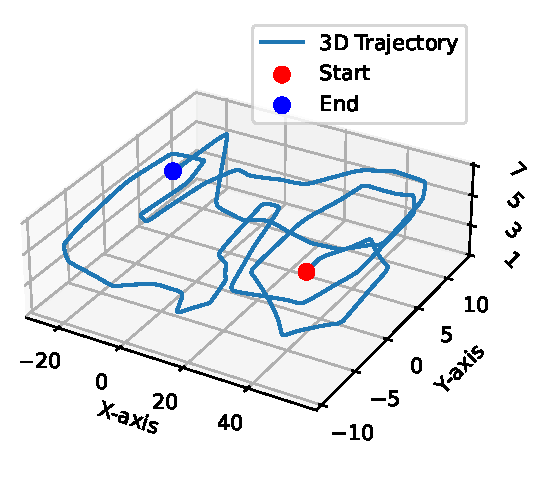
\includegraphics[width=\textwidth]{tex/ch5_airio/figs/pegasus_trajs/pegasus_6_train_test_sorted.pdf}
        \caption{TEST\_3: This trajectory covers a  distance of 402.1$\si{\meter}$ and a total duration of 148.8$\second$, with a peak speed of 4.9 $\si{\meter\per\second}$, an average speed of 2.7 $\si{\meter\per\second}$}
        \label{fig:airio:sub_test3}
    \end{subfigure}
    \caption{Testing set}
    \label{fig:airio:testmain}

\end{figure}
